\documentclass{article}


%%% PAGE DIMENSIONS
\usepackage{geometry} % to change the page dimensions
\geometry{letterpaper} % or letterpaper (US) or a5paper or....
% \geometry{margins=2in} % for example, change the margins to 2 inches all round
% \geometry{landscape} % set up the page for landscape
%   read geometry.pdf for detailed page layout information

\usepackage{graphicx} % support the \includegraphics command and options
%\usepackage{savetrees}
% \usepackage[parfill]{parskip} % Activate to begin paragraphs with an empty line rather than an indent

%%% PACKAGES
\usepackage[round]{natbib}
\usepackage[utf8]{inputenc} % set input encoding (not needed with XeLaTeX)
%\usepackage{listings}
%\usepackage[scaled]{beramono}
%\usepackage[T1]{fontenc}
\usepackage{xcolor}
\usepackage{booktabs} % for much better looking tables
\usepackage{array} % for better arrays (eg matrices) in maths
\usepackage{paralist} % very flexible & customisable lists (eg. enumerate/itemize, etc.)
\usepackage{verbatim} % adds environment for commenting out blocks of text & for better verbatim
\usepackage{subfig} % make it possible to include more than one captioned figure/table in a single float
\usepackage{wrapfig}
\usepackage{algorithm} 
\usepackage{algorithmic}

\usepackage[font={footnotesize}]{caption}
\usepackage[compact]{titlesec}
\titleformat{\subsubsection}[runin]{\normalfont\bfseries}{\thesubsection.}{3pt}{}


% These packages are all incorporated in the memoir class to one degree or another...
%\usepackage{algorithm}
%\usepackage{algpseudocode}
%\usepackage{amsmath}
%\usepackage{amsthm}

%%% HEADERS & FOOTERS
%\usepackage{fancyhdr} % This should be set AFTER setting up the page geometry
%\pagestyle{fancy} % options: empty , plain , fancy
%%\renewcommand{\headrulewidth}{0pt} % customise the layout...
%\lhead{}\chead{}\rhead{}
%\lfoot{}\cfoot{\thepage}\rfoot{}

%%% SECTION TITLE APPEARANCE
%\usepackage{sectsty}
%\allsectionsfont{\sffamily\mdseries\upshape} % (See the fntguide.pdf for font help)
% (This matches ConTeXt defaults)

%%% ToC (table of contents) APPEARANCE
%\usepackage[nottoc,notlof,notlot]{tocbibind} % Put the bibliography in the ToC
%\usepackage[titles,subfigure]{tocloft} % Alter the style of the Table of Contents
%\renewcommand{\cftsecfont}{\rmfamily\mdseries\upshape}
%\renewcommand{\cftsecpagefont}{\rmfamily\mdseries\upshape} % No bold!

%%% END Article customizations
\raggedbottom
%%% The "real" document content comes below...
\linespread{0.9}
\title{VHASH: Spatial DHT based on Voronoi Tessellation}
\author{}
\date{} % Activate to display a given date or no date (if empty),
         % otherwise the current date is printed 


\hyphenation{op-tical net-works semi-conduc-tor Chord-Reduce Map-Reduce Data-Nodes Name-Nodes}
%\KEYWORD{MapReduce; P2P; Parallel Processing; Peer-to-Peer Computing; Cloud Computing; Middleware;}
\begin{document}
%\lstset{language=Python, basicstyle= \footnotesize\ttfamily ,showstringspaces=false, frame=single, commentstyle=\itshape\color{gray}, identifierstyle=\color{black},  keywordstyle=\bfseries\color{red!40!black}, stringstyle=\color{blue}} 



\maketitle
\vspace*{-0.6in}
\begin{abstract}
%1. State the problem
Distributed Hash Tables are used as a tool to generate overlay networks for P2P networks. Current DHT techniques are not designed to take the nature of the underlying network into account when organizing the overlay network; they assign nodes locations in a ring or tree, limiting the ability of these networks to be more efficient. We present VHASH as a spatial DHT based on approximate Delunay Triangulation to integrate location information of nodes into overlay network topology. VHASH allows for the creation of P2P networks with faster record look-up time, storage, and maintenance with a geographically diverse set of nodes.
\end{abstract}


%\begin{IEEEkeywords}
%MapReduce; P2P; Parallel Processing; Peer-to-Peer Computing; Cloud Computing; Middleware;

%\end{IEEEkeywords}
\subsubsection*{VHash}



VHash was created to allow for spacial representations to be mapped to hash locations guided by previous work into object location embedding \citep{voronet}. Rather than focus on minimizing the amount of hops required to travel from point to point we wish to minimize the time required for a message to reach its recipient. VHash actually has a worse worst case hop distance ($O(\sqrt[d]{n})$) than other comparable distributed hash tables ($O(lg(n))$) \citep{chord}. However, VHash can route messages as quickly as possible rather than traveling over a grand tour that an overlay network may describe in the real world. In addition, Vhash offers routing with constant size memory, as average degree in a metric space is defined as a function of the number of dimensions (8 for a 2 dimensions). 


%The intent is that meaning can be ascribed to locations in the DHT and facilitate more efficent function. 
%Specifically in this example we seek to build a minimal latency overlay network for the DHT so a global scale DHT is viable and efficent. 

\begin{wrapfigure}{l}{0.5\textwidth}
\begin{minipage}{0.5\textwidth}

\begin{figure}[H]
\vspace{-30pt}
    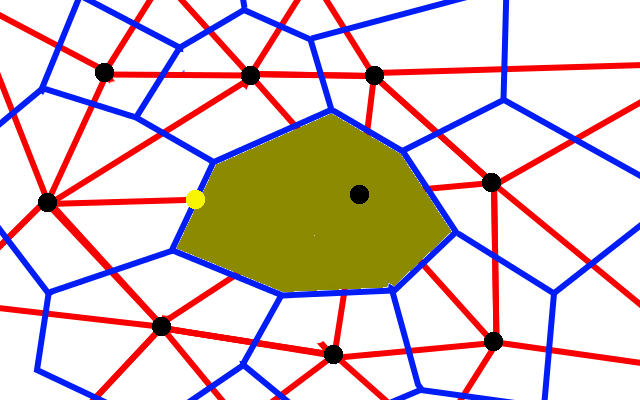
\includegraphics[width=\linewidth]{voronoi-churn4}

    \caption
{
Here, a new node is joining the networks and has established that his position falls in the the yellow shaded Voronoi region.}
\end{figure}
    \end{minipage}
  \end{wrapfigure}



\subsubsection*{Mechanism}
VHash maps nodes to a $d$ dimension toroidal unit space overlay. This is essentially a hypercube with wrapping edges. The toroidal property makes visualization difficult but allows for a space without a sparse edge, as all nodes can translate the space such that they are at the center of the space.  This is a helpful property in ensuring efficient routing to all other nodes.

VHash nodes are responsible for the address space defined by their Voronoi region. This region is defined by a list of peers maintained by the node. A minimum list of peers is maintained such that the node's Voronoi region is well defined. The links connecting the node to its peers correspond to the links of a Delaunay Triangulation.


\begin{wrapfigure}{l}{0.5\textwidth}
\begin{minipage}{0.5\textwidth}
\vspace{-45pt}
\begin{algorithm}[H]

\caption{Vhash Routing}
\label{routing}
{\footnotesize
\begin{algorithmic}[1]  % the number is how many 
	\STATE $P_0$ is this node's set of peers
    \STATE $N$ is this node
	\STATE $m$ is a message addressed for $L$
    \STATE $Forwards$ is the set $P_0\cup{}N$
    \STATE find $C$: member of $Forwards$ which has the shortest distance to $L$
    \IF{$C$ is $N$}
    	\STATE $N$ is the responsible party.
        \STATE Handle $m$
    \ELSE
    	\STATE Forward $m$ to $C$ for handling or further routing
    \ENDIF
\end{algorithmic}
}
\end{algorithm}

\end{minipage}
\end{wrapfigure}
\subsubsection*{Message Routing}





When routing a message to an arbitrary location, a node calculates who's Voronoi region the message's destination is within among the itself and its peers. If the destination falls within its own region, then it is responsible and handles the message accordingly. Otherwise, it forwards the message to the responsible peer and that peer attempts to route the message. This process mimics a pre-computed A* \citep{astar} routing algorithm over the network. 

In terms of metric length, the average routing distance in Vhash is the width of the metric space. A standard DHT overlay is necessarily $O(lg(n))$ as the distance it takes for the DHT to route 1 hop is equivalent to the distance a Vhash message requires to reach the destination. 

\subsubsection*{Joining and Maintenance}
Joining the network is a straightforward process. A new node first learns the location of at least one member of the network to join. The joining node then chooses a location in the hash space either at random or based on a problem formulation (such as geographic location or latency).


After choosing a location, the joining node sends a "join" message to its own location via the known node.
The message is forwarded to the current owner of that location, the "parent" node.
The parent node replies with a maintenance message containing its full peer list. The joining node uses this to begin defining the space for which it is responsible. 
The parent adds the new node to its own peer list and removes all his peers occluded by the new node.  Regular maintenance propagates the new node's information and repairs the overlay topology. 



\begin{wrapfigure}{r}{0.5\textwidth}
\begin{minipage}{0.5\textwidth}
\vspace{-25pt}
\begin{algorithm}[H]
\caption{VHash Greedy Peer Selection}
\label{peer}
{\footnotesize

\begin{algorithmic}[1]  % the number is how many 
	\STATE $Candiates$ is the set of candidate peers
    \STATE $Peers$ is the set of this node's peers
    \STATE $Canidates$ is sorted by each node's closeness to this node
    \STATE The closest member of $Canidates$ is popped and added to $Peers$
    \FORALL{$n$ in $Canidates$}
    	\STATE $c$ is the midpoint between this node and $n$
        \IF{Any node in $Peers$ is closer to $c$ than this node}
        	\STATE reject $n$ as a peer
        \ELSE
        	\STATE Add $n$ to $Peers$
        \ENDIF
    \ENDFOR
\end{algorithmic}
}
\end{algorithm}
\vspace{-30pt}
    \end{minipage}
  \end{wrapfigure}


Each node in the network performs maintenance periodically by a maintenance message to its peers. The maintenance message consists of the node's information and the information on that node's peer list. When a maintenance message is received, the receiving node considers the listed nodes as candidates for its own peer list and removes any occluded nodes. 


\subsubsection*{Data Storage}
Resources in the network, be it raw data or assigned tasks, are assigned hash locations. The node responsible for a given hash location is responsible for the maintenance of that resource. When a node fails, its peers take responsibility of its space. Thus it is important to provide peers with frequent backups of a node's assigned resources.  That way, when a node fails, its peers can immediately assume its responsibilities.

A resource is accessed by contacting the node responsible for the resource.  However, the requester generally has no idea which node is responsible for any particular resource.  The data request message is addressed to the location corresponding to the resource, rather than the node responsible for that location.  The message is forwarded over the overlay network, each hop bringing the node closer until it reaches the responsible node, who sends the resource or an error if the resource does not exist.

\subsubsection*{Conclusion} 
Vhash presents a technique for creating a DHT which allows for efficient optimization of latency and throughput on a Peer to Peer network. It does so by minimizing real routing distance rather than the number of hops. It will facilitate new faster, more efficient DHT based systems.
  
  


{\footnotesize
\bibliographystyle{plainnat}
\bibliography{P3DNS}
}
\end{document}